\documentclass{article}
\usepackage{iclr2026_conference,times}

\input{math_commands.tex}

\usepackage{amsmath}
\usepackage{amssymb}
\usepackage{graphicx}
\usepackage{hyperref}
\hypersetup{
  colorlinks=false,
  pdfborder={0 0 1},
  citebordercolor={0 1 0},
  linkbordercolor={1 0 0},
  urlbordercolor={0 1 0}
}
\usepackage{url}
\usepackage{booktabs}
\usepackage{array}

\title{Counterfactual Grasp Failure Fields}

\author{Anonymous Authors}

\newtheorem{proposition}{Proposition}
\newcommand{\field}{\mathcal{F}}
\newcommand{\success}{\mathcal{S}}
\newcommand{\actions}{\mathcal{A}}
\newcommand{\cost}{c}
\newcommand{\state}{x}
\newcommand{\edit}{\delta}
\newcommand{\score}{\phi}

\begin{document}

\maketitle

\begin{abstract}
Robot grasp failures are often stored as terminal labels: success, failure, slip, low quality, or a scalar confidence score. Such labels are useful for prediction, but they discard the contact-level intervention that would have made the realized grasp work. This paper studies \emph{counterfactual grasp failure fields}: for a failed tactile/contact state, the field is the lowest-cost physically executable edit to contact locations or forces that crosses a mechanical success boundary. The contribution is a representational and diagnostic claim, not a hardware claim. We begin with a two-contact planar pinch model in which paired failures can have identical scalar failure scores while requiring opposite signed contact repairs. We then generalize the experiment to a linear contact-balance family with two to six contact coordinates, unequal contact weights, repair costs, active-contact masks, travel limits, biased repair-sign distributions, and noisy or mismatched margin estimates. The final evidence includes 253,080 streamed baseline evaluations. In the balanced linear contact grid, scalar magnitude-only repair succeeds in 48.9--50.3\% of cases, while the counterfactual field and signed-margin projection succeed in 100.0\%. In biased distributions, a scalar global-sign rule reaches 95.1\% average success at a 0.95 positive-sign prior but has 0.0\% worst-group success. In the large stress suite, the constrained field and signed-margin projection reach 96.0\% success; the missing 4.0\% is not hidden, but reported as actuator/mask infeasibility. Greedy nearest-contact repair reaches 79.4\%, uniform signed repair 63.3\%, scalar random sign 46.9\%, and scalar global sign 68.3\% with 0.0\% worst-group success. The paper's final claim is therefore narrow: scalar terminal labels and scalar magnitude scores are insufficient repair objects because they erase executable direction, allocation, and feasibility information. Signed calibrated mechanics can recover the field in this linear model; the field representation makes that repair object explicit, auditable, and testable under contact constraints.
\end{abstract}

\section{Introduction}

Grasping systems are very good at producing scores. A candidate grasp can be assigned a force-closure quality, a wrench-space metric, a network confidence, a slip probability, or a binary success label. Those scores are valuable before contact. They help select grasp poses, rank proposals, and train perception models. But after the robot has already touched the object, the controller needs a different kind of object. It does not merely need to know that the grasp failed. It needs to know which contact should move, in which direction, by how much, and whether that edit is physically executable.

This paper argues that a realized contact failure should be represented as a \emph{counterfactual grasp failure field}. The field maps a failed contact state to a minimum-cost contact edit that would cross a mechanical success boundary. The variables of the field are not image pixels or latent features. They are contact variables: local contact positions, normal loads, tangential tractions, frictional patches, or active contact sets. The intended use is not only explanation after the fact. The intended use is repair: a controller can attempt the field, reject it if infeasible, or use its infeasibility as a reason to regrasp.

The original short version of this paper made the point in the smallest possible model: a symmetric planar pinch with two contact-height variables. In that toy model, a scalar failure score based on absolute wrench-balance error cannot distinguish two failures that need opposite signed repairs. The analytic counterfactual field repairs all feasible failures in one step, while scalar magnitude-only sign guesses remain near chance. That counterexample is crisp, but it is not enough for a final paper. A hostile reader can correctly say that a signed mechanical margin recovers the same projection. A second hostile reader can say that the two-contact field is only a signed scalar, not a contact field. A third can ask what happens when contacts are blocked, limits are tight, data are biased, or the margin estimate is noisy.

We therefore expand the evidence in four directions. First, we generalize the mechanics to a linear contact-balance family. The success set is an interval in a signed balance coordinate, but the repair variables are multiple contact coordinates with unequal leverage, unequal repair costs, active-contact masks, and travel limits. In this family, the counterfactual field is a weighted projection under constraints. Second, we compare stronger baselines. In addition to scalar random and scalar global-sign repair, we include scalar prior sampling, uniform signed repair, greedy nearest-contact repair, noisy signed-margin projection, exact signed-margin projection, and the constrained counterfactual field. Third, we report distributional failures: scalar majority rules can look excellent on average under biased repair signs while failing every minority-sign case. Fourth, we treat infeasibility as a result. If the active contacts and limits cannot execute the edit, the field should say so rather than pretending repair succeeded.

The result is deliberately nuanced. The field does not beat exact signed mechanics in the linear model. It should not: the exact signed margin plus calibrated contact allocation contains the same information. This is a feature of the paper, not a weakness to hide. The claim is not that every scalar-valued mechanical method is doomed. The claim is that terminal labels and scalar magnitude scores are the wrong repair object. A calibrated signed margin can be used to compute the field; the field is the executable object that should be stored, learned, evaluated, and audited.

The paper makes four contributions:
\begin{itemize}
    \item a formal definition of counterfactual grasp failure fields as minimum-cost executable contact edits;
    \item a scalar-insufficiency proposition for identical scalar failure scores with opposite repairs;
    \item a full-scale linear contact-balance simulation with 253,080 streamed baseline evaluations across contact count, distribution bias, actuator masks, limits, noise, and stress randomization;
    \item an honest claim audit showing where scalar labels fail, where signed mechanics recovers the field, and where the field itself becomes infeasible.
\end{itemize}

\section{Related Work And Novelty Boundary}

\paragraph{Grasp mechanics and grasp quality.}
Analytic grasping represents stability through contact geometry, friction cones, force closure, and wrench-space quality \citep{ferrari1992planning,bicchi2000robotic,roa2015grasp}. Large-scale data-driven grasping systems often use these criteria or empirical outcomes as training labels \citep{mahler2017dexnet}. This paper does not claim new grasp mechanics. It uses simple mechanics as a success boundary and asks what object should be represented after a realized failure. A grasp quality score asks whether a candidate is good. A counterfactual field asks what physical contact edit would have made a specific failed state good.

\paragraph{Tactile stability, slip, and regrasping.}
Tactile sensors can measure contact shape, shear, slip, and force distributions \citep{yuan2015measurement,lambeta2020digit}. Tactile servoing and regrasp systems can react to slip or transform tactile observations into corrective actions \citep{chebotar2016bigs,veiga2018grip,hogan2018tactile,hogan2020tactile}. These works are close in spirit because they care about repair, not only prediction. The distinction here is representational: we isolate the target object that a repair system should predict or optimize. A tactile policy may implicitly learn a useful correction, but if its supervision is only a scalar failure label, the direction and allocation of the repair are not first-class quantities.

\paragraph{Counterfactual explanations.}
Counterfactual explanations ask which input changes would flip a model decision \citep{pearl2009causality,wachter2017counterfactual}. Generic counterfactual feature edits are not enough for grasp repair because an edited feature may not be a physically executable contact action. Our definition restricts the action space to contact edits and judges the edit by a mechanical success predicate. The paper is therefore closer to constrained counterfactual control than to post hoc explanation of a classifier.

\paragraph{Hostile boundary.}
There are three important hostile interpretations. The first is ``this is just a grasp-quality gradient.'' In the linear model, a signed calibrated margin does recover the field, and the experiments report that upper bound. The second is ``this is just tactile servoing.'' Tactile servoing is a control strategy; the field is the contact-level repair target that such a strategy may use. The third is ``force closure already solves it.'' Force closure scores a state or candidate grasp; the field gives the minimum executable edit from a failed state to the success set. The novelty is not broad mechanics. It is the insistence that repair evidence be represented as a contact-indexed counterfactual object rather than a scalar terminal label.

\section{Counterfactual Failure Fields}

Let $\state$ be a realized tactile/contact state and let $\success$ be the set of states satisfying a mechanical success predicate. Let $\actions(\state)$ be the set of physically executable contact edits at that state. A counterfactual grasp failure field is
\begin{equation}
    \field(\state) \in
    \arg\min_{\edit \in \actions(\state)}
    \cost(\edit)
    \quad
    \mathrm{s.t.}
    \quad
    \state+\edit \in \success.
    \label{eq:field}
\end{equation}
If the set of minimizers is non-unique, the honest object is a repair set. In this paper we use a weighted Euclidean cost, so the linear cases have a unique minimum unless the action set is infeasible. The definition is intentionally modest. It does not say the robot can always execute the field. It says the repair object should carry direction, allocation, effort, and infeasibility.

\subsection{The Original Planar Pinch}

Consider two opposing point contacts on a planar object. The left contact is at $(-a,y_L)$ with force $(N,t_L)$ and the right contact is at $(a,y_R)$ with force $(-N,t_R)$, where $N>0$ is the normal force and $|t_i|\leq \mu N$ are tangential friction constraints. The grasp must resist a vertical load $W$ and external torque $\tau$. Quasi-static balance gives
\begin{equation}
    t_L+t_R=W,
    \quad
    -a t_L + a t_R + N(y_R-y_L)=\tau .
\end{equation}
Writing $d=t_R-t_L$, feasibility is equivalent to
\begin{equation}
    |d|\leq 2\mu N-W,
    \quad
    d=\frac{\tau-N(y_R-y_L)}{a}.
\end{equation}
Therefore the contact state succeeds when
\begin{equation}
    |e|\leq h,
    \quad
    e=\frac{\tau}{N}-(y_R-y_L),
    \quad
    h=\frac{a(2\mu N-W)}{N}.
    \label{eq:interval}
\end{equation}
For a failed state $|e|>h$, the minimum Euclidean displacement that reaches the nearest boundary is
\begin{equation}
    g=e-\operatorname{sign}(e)h,
    \quad
    \delta_R=\frac{g}{2},
    \quad
    \delta_L=-\frac{g}{2}.
    \label{eq:closedform}
\end{equation}
The repair is small, but it already contains what a scalar failure magnitude discards: the sign of the contact-height difference change.

\begin{proposition}[Scalar magnitude is insufficient for deterministic repair]
Fix $r>h$ and two failed states $\state_+$ and $\state_-$ with errors $e(\state_+)=r$ and $e(\state_-)=-r$. Let $\score(\state)=\psi(|e(\state)|)$ be any scalar representation identical for equal absolute error. Any deterministic repair rule $\pi(\score(\state))$ assigns the same contact edit to $\state_+$ and $\state_-$. The minimum-norm stabilizing fields for the two states require opposite signs of $\delta_R-\delta_L$. Therefore $\pi$ cannot equal the minimum stabilizing field on both states.
\end{proposition}

\noindent\textbf{Proof.}
Since $|e(\state_+)|=|e(\state_-)|$, the scalar representations are identical. A deterministic rule must return the same edit. Equation~\ref{eq:closedform} gives required difference changes $r-h$ and $-(r-h)$, which have opposite signs. One signed edit cannot be the minimum repair for both. \hfill $\square$

\subsection{A Linear Contact-Balance Family}

The full-scale experiments use a broader linear family. A contact state has $m$ editable contact coordinates $y\in\R^m$, a signed target $b$, contact leverage weights $w\in\R^m$, positive repair costs $c_i$, travel limits $\ell_i$, and active-contact indicators $a_i\in\{0,1\}$. The signed balance error is
\begin{equation}
    e=b-w^\top y.
\end{equation}
The state succeeds when $|e|\leq h$. For a failed state, the desired balance change is
\begin{equation}
    g=e-\operatorname{sign}(e)h.
\end{equation}
The unconstrained weighted field solves
\begin{equation}
    \min_{\delta}\sum_i c_i\delta_i^2
    \quad \mathrm{s.t.}\quad
    w^\top\delta=g,
\end{equation}
with solution
\begin{equation}
    \delta_i =
    \frac{g\,w_i/c_i}{\sum_j w_j^2/c_j}.
    \label{eq:weighted}
\end{equation}
When active masks and travel limits are present, the feasible action set adds
\begin{equation}
    \delta_i=0 \quad \mathrm{if}\quad a_i=0,
    \qquad
    |y_i+\delta_i|\leq \ell_i.
\end{equation}
The full-scale runner solves this one-constraint box-constrained projection with a small active-set routine. If the constraint cannot be satisfied by the active contacts within their limits, the field is marked infeasible.

\begin{proposition}[Signed calibrated margins recover the field in the linear model]
In the unconstrained linear contact-balance family, a method with access to the signed error $e$, radius $h$, weights $w$, and costs $c_i$ recovers the counterfactual field by Equation~\ref{eq:weighted}. With active masks and travel limits, the same information plus the action constraints recovers the constrained projection or certifies infeasibility.
\end{proposition}

This proposition is the reason the paper does not claim dominance over signed mechanics. If the robot has a calibrated signed margin and a correct contact-action model, it has the information needed to compute the field. The field is still the right repair object: it is the vector edit, effort, and feasibility certificate produced from that information.

\section{Baselines}

Table~\ref{tab:baseline-access} records the information budget for each baseline. The baselines are deliberately ordered from scalar-only to full contact-field access.

\begin{table}[t]
    \centering
    \caption{Baseline information access. The field is not compared only against weak scalar guesses; it is also compared against signed-margin and contact-aware repair rules.}
    \label{tab:baseline-access}
    \small
    \begin{tabular}{lll}\toprule
Baseline & Uses sign? & Uses contact allocation?\\
\midrule
no repair & no & no\\
scalar random sign & guessed & generic\\
scalar global sign & prior only & generic\\
uniform signed & yes & no\\
nearest contact & yes & greedy\\
noisy signed margin & noisy & estimated\\
signed margin & yes & yes\\
counterfactual field & yes & yes, constrained\\
\bottomrule\end{tabular}

\end{table}

\paragraph{No repair.}
The no-repair baseline applies $\delta=0$. It verifies that all sampled cases are actually failures.

\paragraph{Scalar random sign.}
This baseline knows only failure magnitude $|e|-h$ and guesses the missing sign uniformly at random. It receives the generic contact allocation formula after the sign guess, so it is generous to scalar magnitude.

\paragraph{Scalar global sign.}
This baseline always chooses the majority repair sign implied by the data distribution. It is the baseline most likely to look good on biased data while failing all minority-sign repairs.

\paragraph{Scalar prior sample.}
This baseline samples the sign from the known sign prior. It can match the marginal distribution but still does not know which realized failure belongs to which sign.

\paragraph{Uniform signed repair.}
This baseline receives the correct sign but spreads the repair uniformly over active contacts. It tests whether knowing direction without allocation is enough.

\paragraph{Nearest-contact repair.}
This baseline receives the correct sign and moves the highest-leverage active contact. It is a greedy contact-aware baseline.

\paragraph{Noisy signed margin.}
This baseline receives a signed margin and contact weights corrupted by relative noise. It tests whether a field computed from imperfect mechanics remains reliable.

\paragraph{Signed-margin projection.}
This is the strongest analytic upper bound. It receives the true signed error, weights, costs, active contacts, and limits. In the linear model it should match the field exactly.

\paragraph{Counterfactual field.}
This baseline is the constrained minimum-cost field from Eq.~\ref{eq:field}. It reports infeasibility when active contacts and limits cannot realize the required balance change.

\section{Experimental Protocol}

All experiments are generated by \path{experiments/run_full_scale_fields.py}. The runner streams compact per-baseline rows to CSV files under \path{results/full_scale/}, writes generated figures under \path{results/full_scale/figures/}, copies paper-ready figures to \path{paper/figures/}, and writes table fragments to \path{paper/tables/}. It stores no raw trajectories.

\paragraph{Existing v2 reproduction.}
The original runner \path{experiments/run_counterfactual_fields.py} with \texttt{--n 20000 --seed 2} is retained. It samples 20,000 feasible failed states in the symmetric pinch model and a 30-seed stress suite with 3,000 cases per seed.

\paragraph{Linear contact grid.}
The linear contact grid evaluates contact counts $m\in\{2,3,4,6\}$ with randomized contact weights, repair costs, limits, and balanced repair signs. It produces 60,480 streamed baseline rows.

\paragraph{Biased scalar grid.}
The biased grid varies the probability of positive repair signs from 0.50 to 0.95. It tests whether average success hides minority-direction failure. It produces 45,000 baseline rows.

\paragraph{Mask and limit grid.}
The mask/limit grid randomly disables contacts and varies travel-limit scale. It intentionally keeps cases where the constrained field can be infeasible. It produces 57,600 baseline rows.

\paragraph{Noise and mismatch grid.}
The noise grid corrupts signed margin and contact weights for the noisy signed-margin baseline. Exact signed margin and field baselines remain oracle references. It produces 36,000 baseline rows.

\paragraph{Large seeded stress suite.}
The stress suite randomizes contact count, repair-sign prior, contact masks, travel limits, near-limit states, and noise settings. It produces 54,000 baseline rows. Across all full-scale suites, the final run writes 253,080 baseline evaluations.

\paragraph{Metrics.}
Success means the repaired state satisfies the balance interval and the contact limits. Balanced success averages positive- and negative-error success rates. Worst-group success is the lower of those two rates. Effort is the weighted norm of the repair. Field infeasible rate reports cases where the true constrained field cannot reach the boundary with available contacts and limits.

\section{Results}

\subsection{Original Symmetric Counterexample}

\begin{figure}[t]
    \centering
    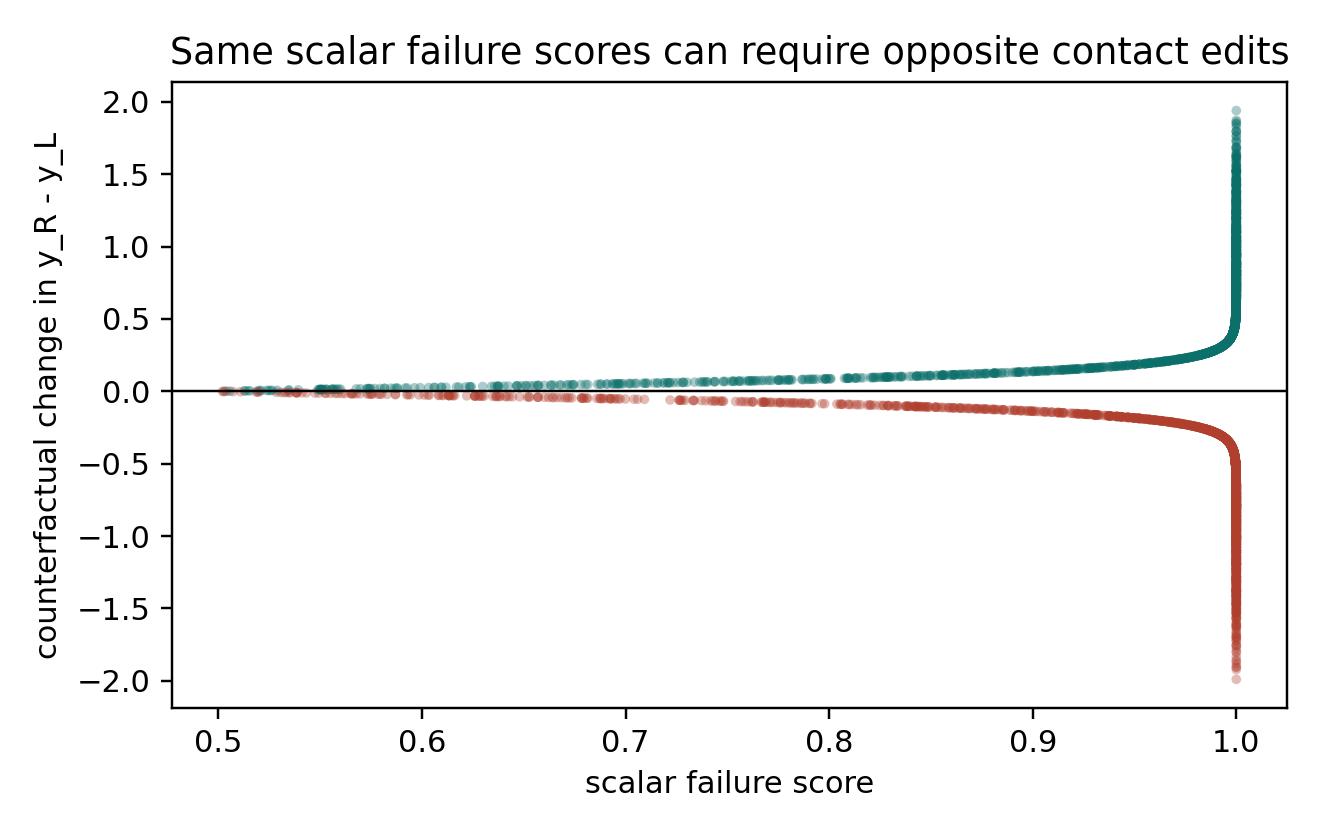
\includegraphics[width=0.48\linewidth]{figures/same_score_opposite_repairs.png}
    \hfill
    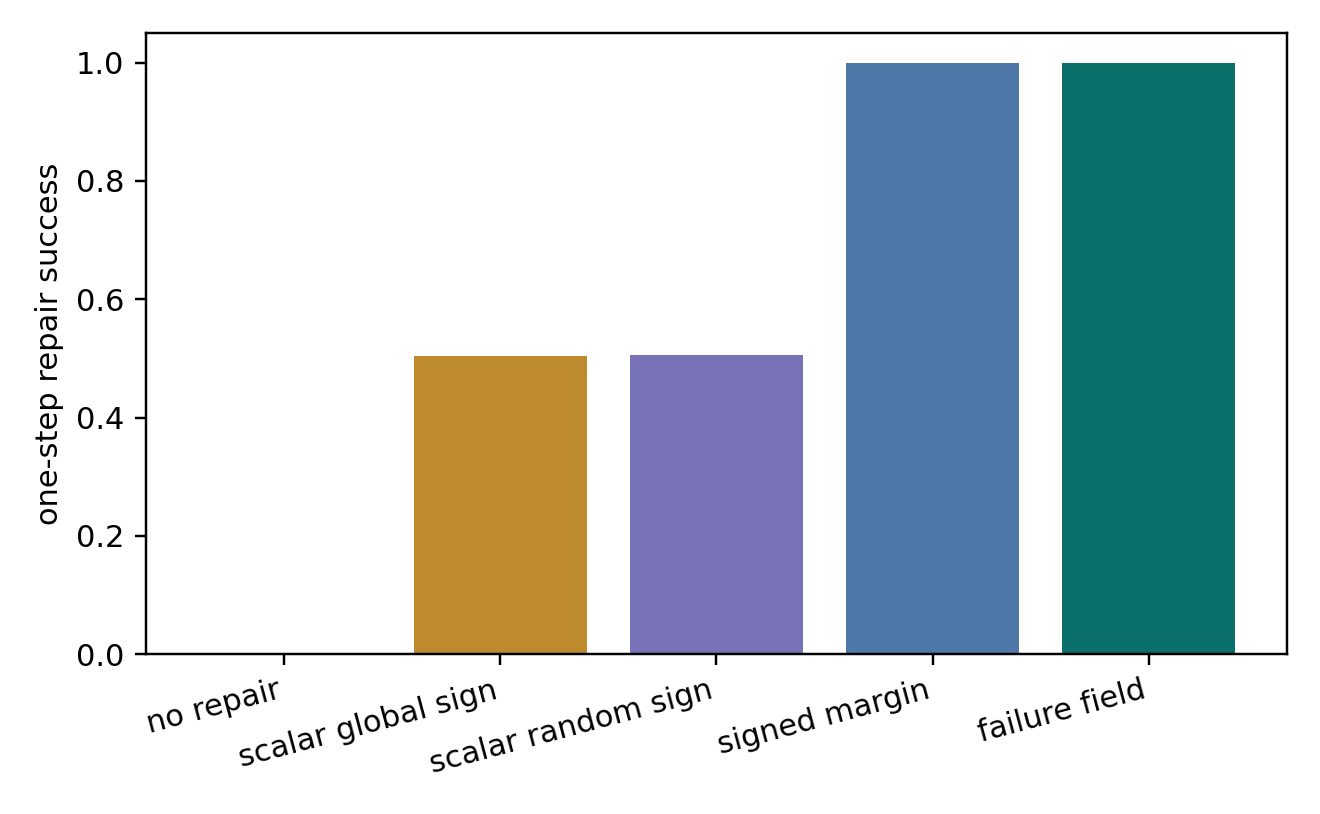
\includegraphics[width=0.48\linewidth]{figures/repair_success_rates.png}
    \caption{Original symmetric pinch evidence. Left: equal scalar failure scores can require opposite contact-difference repairs. Right: the analytic field and signed-margin projection repair all 20,000 feasible failures; scalar sign guesses remain near chance.}
    \label{fig:original}
\end{figure}

The original experiment remains the cleanest counterexample. In 20,000 feasible failed pinches, the field and signed-margin projection both achieve 1.0000 one-step success. Scalar random-sign repair succeeds in 0.5059 of cases and scalar global-sign repair in 0.50415. Repair-sign entropy after scalarization is 0.99995 bits. The paired examples show identical failure scores with opposite required contact edits. This supports the scalar-insufficiency proposition, but only in a symmetric two-contact family.

\begin{figure}[t]
    \centering
    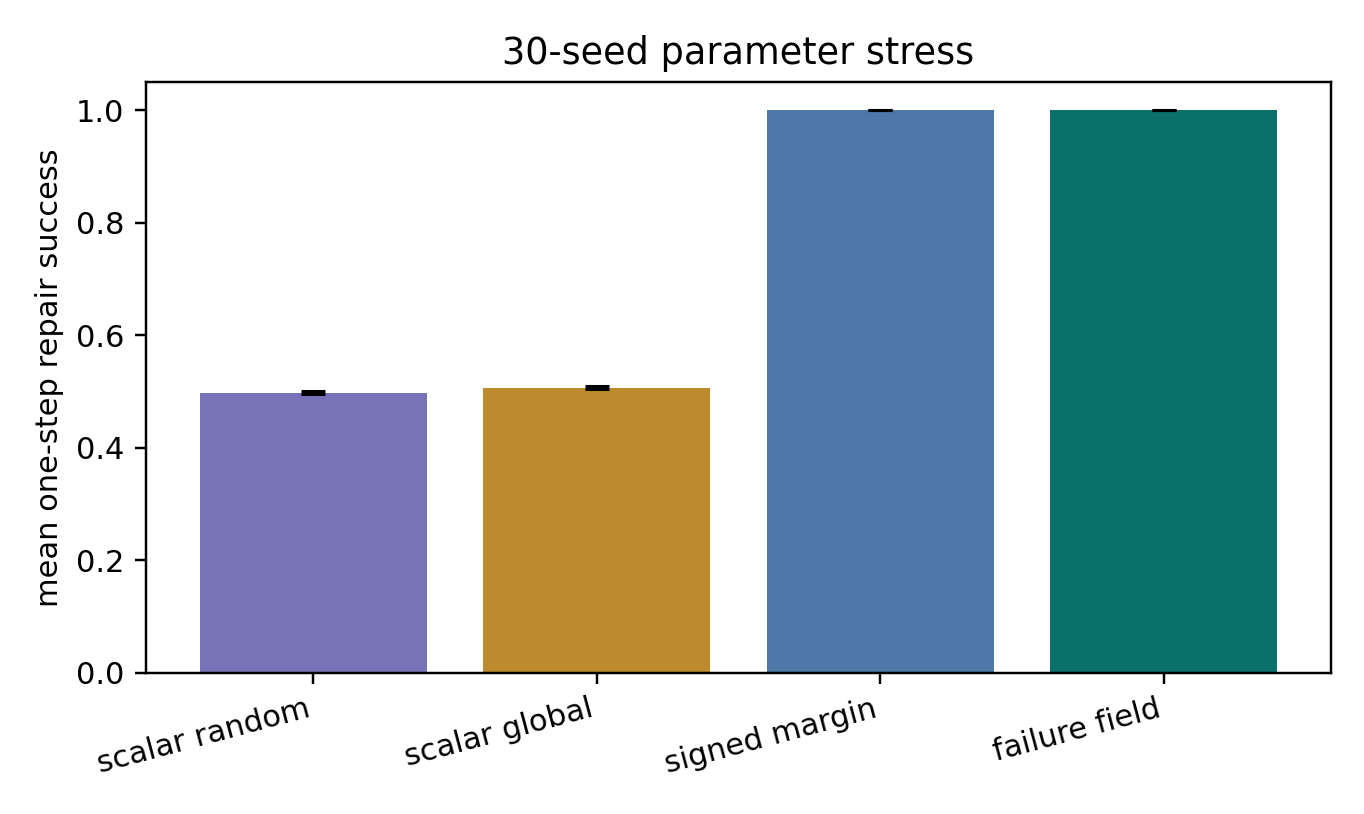
\includegraphics[width=0.62\linewidth]{figures/stress_success_rates.png}
    \caption{Original 30-seed stress test. The field and signed-margin upper bound remain at 1.0 one-step success; scalar magnitude-only repair remains near chance.}
    \label{fig:old-stress}
\end{figure}

The original 30-seed stress suite randomizes half-width, normal force, friction, object weight, and finger travel limit. The field mean one-step success is 1.0, signed margin is 1.0, scalar random sign is $0.4983\pm0.0029$, and scalar global sign is $0.5073\pm0.0020$. The original result therefore survives parameter stress, but it still does not address multi-contact allocation, biased data, or infeasible repairs.

\subsection{Full-Scale Leaderboard}

\begin{figure}[t]
    \centering
    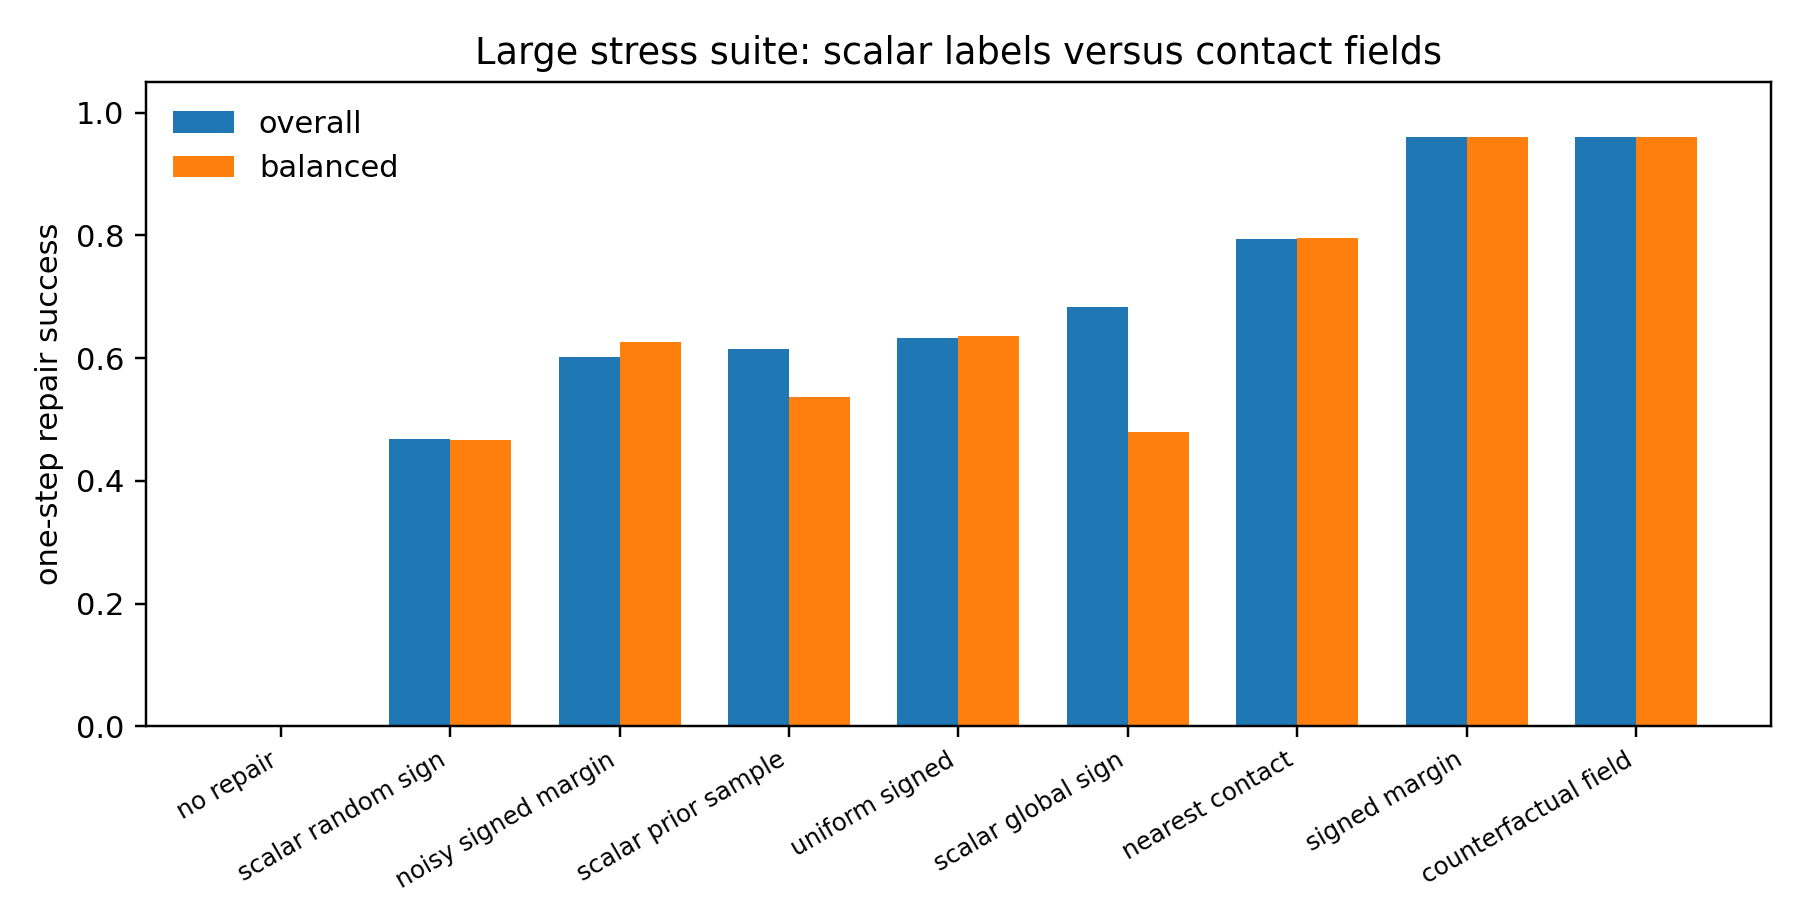
\includegraphics[width=0.92\linewidth]{figures/full_scale_success_leaderboard.png}
    \caption{Large stress-suite success rates. Scalar baselines lose repair direction; uniform and nearest-contact baselines know sign but lose allocation; signed-margin projection and the counterfactual field match because signed calibrated mechanics is sufficient in the linear model.}
    \label{fig:leaderboard}
\end{figure}

Table~\ref{tab:leaderboard} summarizes the full-scale suites. The balanced linear contact grid is the direct generalization of the toy counterexample. Scalar random sign succeeds in 48.9\%, scalar global sign in 49.6\%, and scalar prior sampling in 50.3\%. Uniform signed repair succeeds in 77.7\%, showing that sign alone is not enough when contacts have unequal leverage and cost. Greedy nearest-contact repair reaches 91.6\%, but still fails cases where the minimum repair must be distributed across contacts. The field, exact signed-margin projection, and zero-noise signed-margin baseline reach 100.0\%.

\begin{table}[p]
    \centering
    \scriptsize
    \caption{Full-scale leaderboard. Success is one-step mechanical repair success. Bal. is balanced success over positive and negative repair directions. Worst is worst-group success. Effort is weighted repair norm.}
    \label{tab:leaderboard}
    \resizebox{\linewidth}{!}{\begin{tabular}{llrrrrr}\toprule
Suite & Baseline & $n$ & Success & Bal. & Worst & Effort\\
\midrule
biased scalar grid & scalar random sign & 9000 & 50.8\% & 51.4\% & 50.2\% & 0.18\\
biased scalar grid & scalar global sign & 9000 & 76.3\% & 50.0\% & 0.0\% & 0.18\\
biased scalar grid & signed margin & 9000 & 100.0\% & 100.0\% & 100.0\% & 0.18\\
biased scalar grid & counterfactual field & 9000 & 100.0\% & 100.0\% & 100.0\% & 0.18\\
large seed stress & scalar random sign & 6000 & 46.9\% & 46.7\% & 46.3\% & 0.22\\
large seed stress & scalar global sign & 6000 & 68.3\% & 48.0\% & 0.0\% & 0.23\\
large seed stress & uniform signed & 6000 & 63.3\% & 63.6\% & 63.0\% & 0.63\\
large seed stress & nearest contact & 6000 & 79.4\% & 79.6\% & 79.1\% & 0.24\\
large seed stress & noisy signed margin & 6000 & 60.2\% & 62.7\% & 56.8\% & 0.23\\
large seed stress & signed margin & 6000 & 96.0\% & 96.1\% & 96.0\% & 0.23\\
large seed stress & counterfactual field & 6000 & 96.0\% & 96.1\% & 96.0\% & 0.23\\
linear contact grid & scalar random sign & 6720 & 48.9\% & 48.9\% & 48.5\% & 0.20\\
linear contact grid & scalar global sign & 6720 & 49.6\% & 50.0\% & 0.0\% & 0.20\\
linear contact grid & uniform signed & 6720 & 77.7\% & 77.7\% & 77.6\% & 0.71\\
linear contact grid & nearest contact & 6720 & 91.6\% & 91.6\% & 91.3\% & 0.26\\
linear contact grid & noisy signed margin & 6720 & 100.0\% & 100.0\% & 100.0\% & 0.20\\
linear contact grid & signed margin & 6720 & 100.0\% & 100.0\% & 100.0\% & 0.20\\
linear contact grid & counterfactual field & 6720 & 100.0\% & 100.0\% & 100.0\% & 0.20\\
mask limit grid & uniform signed & 11520 & 36.0\% & 36.0\% & 35.7\% & 0.57\\
mask limit grid & nearest contact & 11520 & 57.2\% & 57.2\% & 56.8\% & 0.17\\
mask limit grid & signed margin & 11520 & 93.5\% & 93.5\% & 93.2\% & 0.21\\
mask limit grid & counterfactual field & 11520 & 93.5\% & 93.5\% & 93.2\% & 0.21\\
noise mismatch grid & scalar random sign & 9000 & 50.3\% & 50.3\% & 49.9\% & 0.18\\
noise mismatch grid & noisy signed margin & 9000 & 55.0\% & 55.0\% & 54.9\% & 0.18\\
noise mismatch grid & signed margin & 9000 & 100.0\% & 100.0\% & 100.0\% & 0.18\\
noise mismatch grid & counterfactual field & 9000 & 100.0\% & 100.0\% & 100.0\% & 0.18\\
\bottomrule\end{tabular}
}
\end{table}

The large stress suite is more realistic for this paper's scope. It includes contact masks and tight limits, so the true field is infeasible in 3.95\% of cases. The field and signed-margin projection both reach 96.0\% success and 96.1\% balanced success. This is not an algorithmic victory of the named field over signed mechanics. It is an accounting victory: the field reports the 4.0\% of cases where no one-step active-contact repair exists. Scalar random sign reaches 46.9\%. Scalar global sign reaches 68.3\% average success but 0.0\% worst-group success. Uniform signed repair reaches 63.3\%, and nearest-contact repair reaches 79.4\%.

\subsection{Biased Data Can Hide Scalar Failure}

\begin{figure}[t]
    \centering
    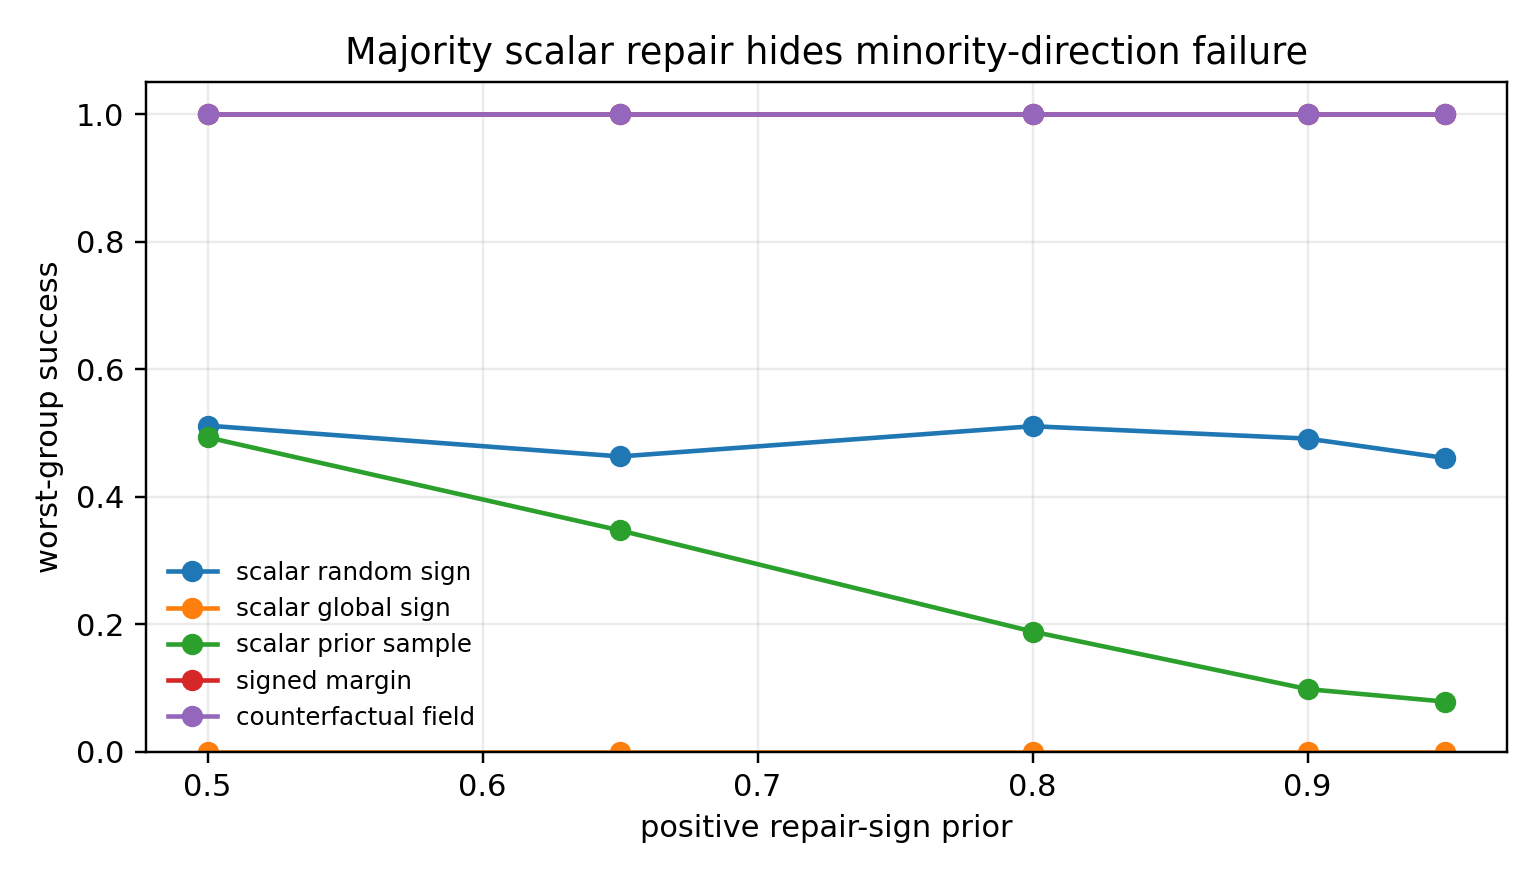
\includegraphics[width=0.82\linewidth]{figures/bias_worst_group_curve.png}
    \caption{Worst-group success under repair-sign bias. A scalar global-sign rule looks strong on average as one repair direction dominates, but it fails every minority-direction case.}
    \label{fig:bias}
\end{figure}

The biased scalar grid explains why average success is not enough. At a 0.95 positive-sign prior, scalar global-sign repair reaches 95.1\% average success. If a paper reported only that number, the scalar repair rule would appear nearly solved. But its balanced success remains 50.0\% and its worst-group success is 0.0\%, because every negative-sign repair is wrong. Scalar prior sampling is less brittle but still poor: at the same 0.95 prior it reaches 90.2\% average success and only 7.9\% worst-group success.

\begin{table}[t]
    \centering
    \scriptsize
    \caption{Biased scalar grid. Majority-sign scalar repair can produce high average success while preserving zero worst-group success.}
    \label{tab:bias}
    \resizebox{\linewidth}{!}{\begin{tabular}{lrrrr}\toprule
Baseline & Prior & Success & Bal. & Worst\\
\midrule
scalar global sign & 0.50 & 51.1\% & 50.0\% & 0.0\%\\
scalar prior sample & 0.50 & 50.4\% & 50.4\% & 49.3\%\\
signed margin & 0.50 & 100.0\% & 100.0\% & 100.0\%\\
counterfactual field & 0.50 & 100.0\% & 100.0\% & 100.0\%\\
scalar global sign & 0.65 & 66.2\% & 50.0\% & 0.0\%\\
scalar prior sample & 0.65 & 54.7\% & 49.8\% & 34.7\%\\
signed margin & 0.65 & 100.0\% & 100.0\% & 100.0\%\\
counterfactual field & 0.65 & 100.0\% & 100.0\% & 100.0\%\\
scalar global sign & 0.80 & 78.8\% & 50.0\% & 0.0\%\\
scalar prior sample & 0.80 & 68.1\% & 50.1\% & 18.8\%\\
signed margin & 0.80 & 100.0\% & 100.0\% & 100.0\%\\
counterfactual field & 0.80 & 100.0\% & 100.0\% & 100.0\%\\
scalar global sign & 0.90 & 90.4\% & 50.0\% & 0.0\%\\
scalar prior sample & 0.90 & 81.9\% & 49.7\% & 9.8\%\\
signed margin & 0.90 & 100.0\% & 100.0\% & 100.0\%\\
counterfactual field & 0.90 & 100.0\% & 100.0\% & 100.0\%\\
scalar global sign & 0.95 & 95.1\% & 50.0\% & 0.0\%\\
scalar prior sample & 0.95 & 90.2\% & 51.2\% & 7.9\%\\
signed margin & 0.95 & 100.0\% & 100.0\% & 100.0\%\\
counterfactual field & 0.95 & 100.0\% & 100.0\% & 100.0\%\\
\bottomrule\end{tabular}
}
\end{table}

This is the key reason the paper reports balanced and worst-group metrics. Many grasp datasets are biased: common objects, common approach directions, gravity, and gripper geometry may make one repair direction more frequent. A scalar label can exploit that bias without representing the repair field. A field representation makes the minority repair direction visible.

\subsection{Contact Allocation Matters}

Knowing the repair sign is useful but insufficient when multiple contacts have unequal leverage, costs, or limits. Uniform signed repair receives the correct sign, but it ignores contact allocation and reaches only 77.7\% in the linear contact grid and 63.3\% in the large stress suite. Nearest-contact repair is stronger because it moves the highest-leverage contact, reaching 91.6\% in the linear grid and 79.4\% in the stress suite. Both baselines fail because the minimum-cost edit often requires a distribution over contacts rather than a single direction.

\begin{figure}[t]
    \centering
    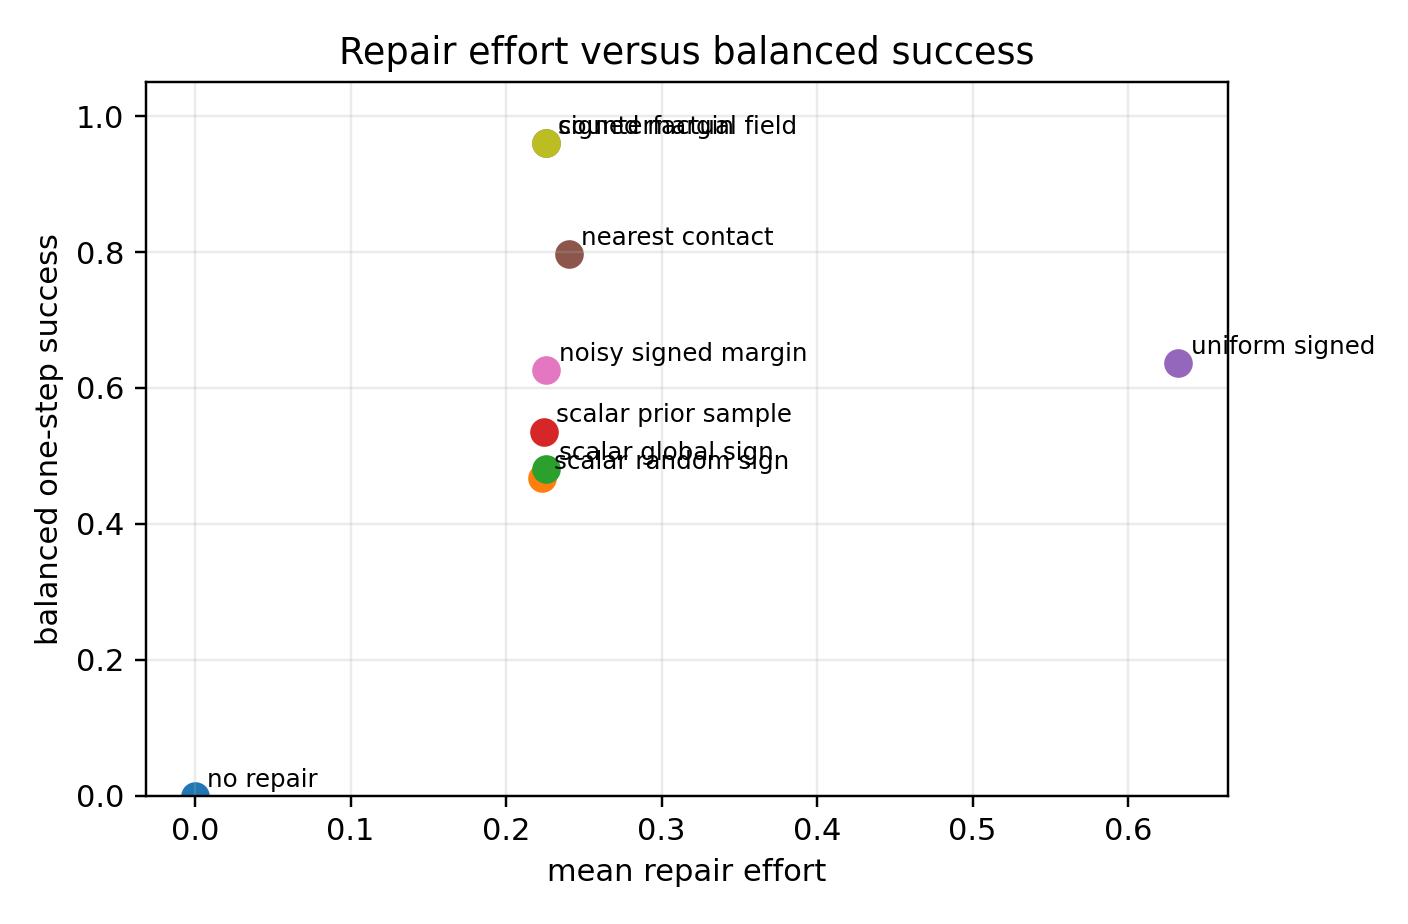
\includegraphics[width=0.62\linewidth]{figures/effort_success_pareto.png}
    \caption{Large stress-suite effort versus balanced success. Nearest-contact repair is a strong heuristic but does not match the constrained field. Uniform repair spends more effort and succeeds less often.}
    \label{fig:pareto}
\end{figure}

Figure~\ref{fig:pareto} shows the effort-success tradeoff. Uniform signed repair spends the most effort and has lower success, because equal motion across contacts is rarely the weighted projection. Nearest-contact repair has moderate effort and better success, but it is still a greedy heuristic. The field and signed-margin projection occupy the intended corner: highest balanced success at moderate effort, limited only by infeasible cases in the stress suite.

\subsection{Active Contacts And Travel Limits}

\begin{figure}[t]
    \centering
    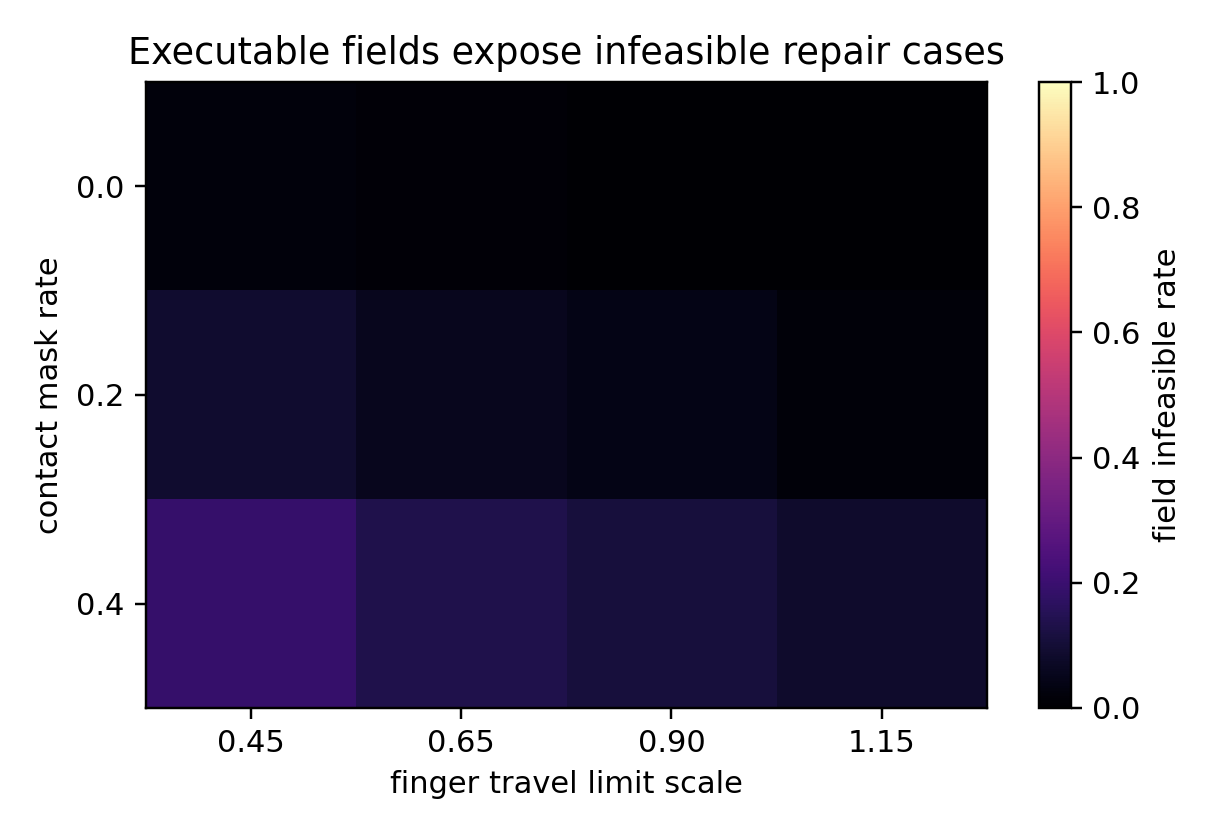
\includegraphics[width=0.74\linewidth]{figures/mask_limit_feasibility_map.png}
    \caption{Field infeasibility under active-contact masks and travel limits. A field representation should report these cases rather than collapsing them into a scalar failure label.}
    \label{fig:mask}
\end{figure}

The mask/limit suite is the most important boundary result. When no contacts are masked and travel limits are generous, the constrained field succeeds in 99.5\% of cases. With 40\% of contacts masked and the tightest travel limit scale, field infeasibility rises to 19.0\% and field success falls to 81.0\%. This does not refute the field representation. It is exactly the information the representation should expose: the one-step contact edit is not executable with the current active contacts.

\begin{table}[t]
    \centering
    \scriptsize
    \caption{Mask/limit feasibility. Field infeasible rate is the rate at which no active-contact edit can reach the boundary within limits.}
    \label{tab:mask}
    \resizebox{0.82\linewidth}{!}{\begin{tabular}{rrrrr}\toprule
Mask & Limit & Field infeasible & Field success & Nearest success\\
\midrule
0.0 & 0.45 & 2.2\% & 97.8\% & 54.4\%\\
0.0 & 0.65 & 1.4\% & 98.6\% & 55.1\%\\
0.0 & 0.90 & 0.6\% & 99.4\% & 59.5\%\\
0.0 & 1.15 & 0.5\% & 99.5\% & 60.6\%\\
0.2 & 0.45 & 9.0\% & 91.0\% & 51.9\%\\
0.2 & 0.65 & 5.8\% & 94.2\% & 53.4\%\\
0.2 & 0.90 & 4.2\% & 95.8\% & 59.4\%\\
0.2 & 1.15 & 1.8\% & 98.2\% & 63.9\%\\
0.4 & 0.45 & 19.0\% & 81.0\% & 48.6\%\\
0.4 & 0.65 & 13.6\% & 86.4\% & 54.8\%\\
0.4 & 0.90 & 11.0\% & 89.0\% & 60.1\%\\
0.4 & 1.15 & 8.5\% & 91.5\% & 64.4\%\\
\bottomrule\end{tabular}
}
\end{table}

The nearest-contact baseline is particularly sensitive to this setting. Even with no mask and loose limits, it succeeds in only about 60\% of mask/limit cases. With 40\% masks and tight limits, it falls below 50\%. Greedy single-contact repairs are attractive for simple controllers, but the result shows why a field should be contact-indexed: the best edit may need several available contacts, and sometimes none are available.

\subsection{Noise And Mismatch}

\begin{figure}[t]
    \centering
    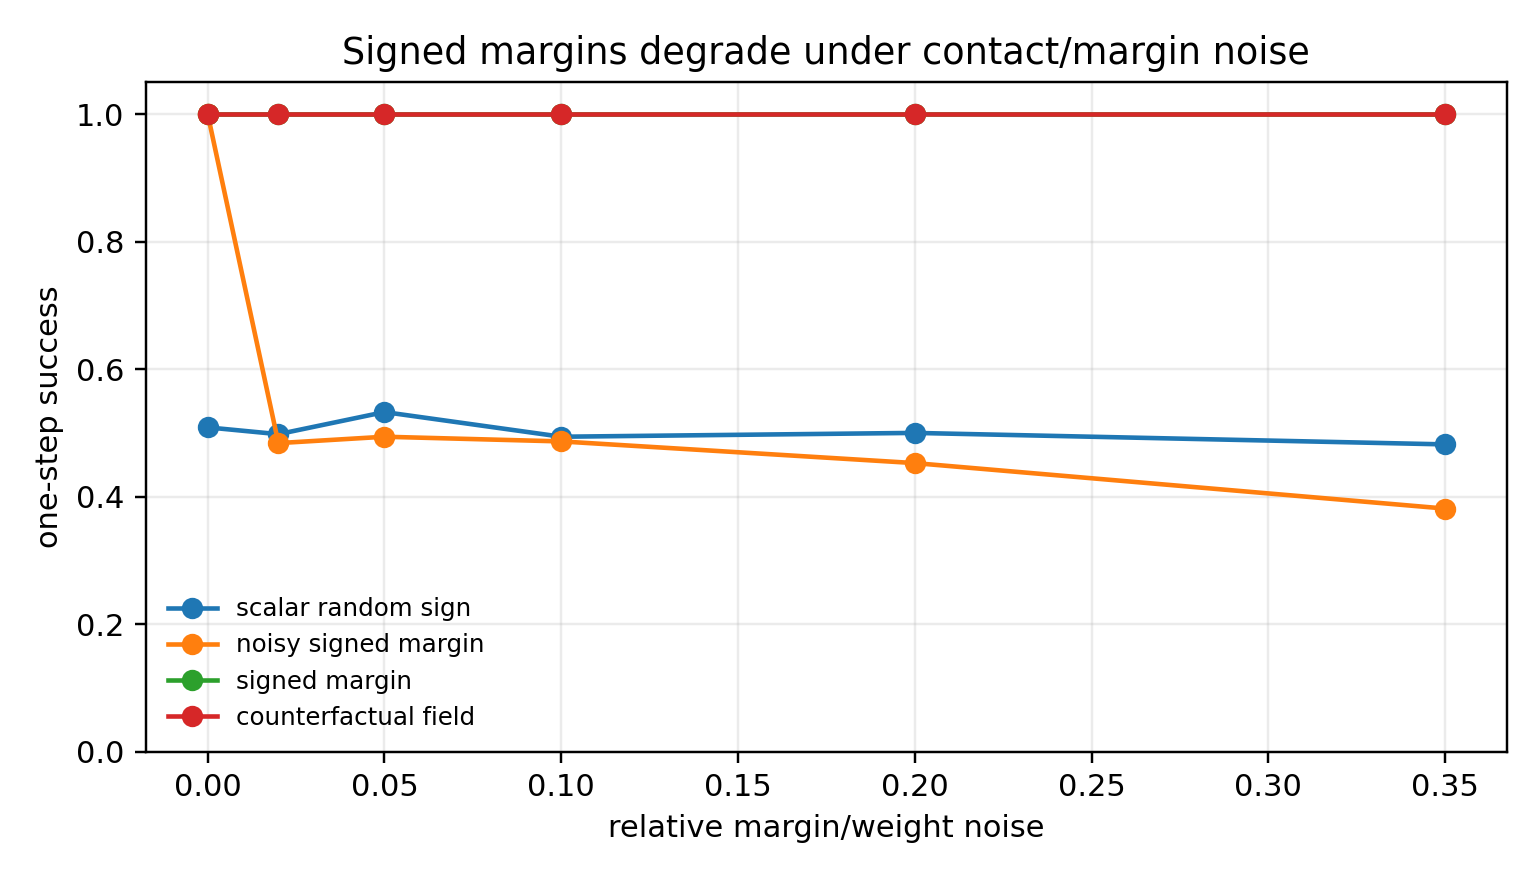
\includegraphics[width=0.82\linewidth]{figures/noise_mismatch_success.png}
    \caption{Noise/mismatch suite. Exact signed mechanics remains an oracle upper bound, but noisy signed margins lose their one-step guarantee because boundary-targeted projections have no slack.}
    \label{fig:noise}
\end{figure}

The noise suite separates exact information from estimated information. With zero noise, noisy signed margin is identical to signed margin and succeeds in 100.0\% of cases. At only 0.02 relative noise, it falls to 48.4\% success in this boundary-targeted one-step metric. At 0.35 noise it falls to 38.1\%. This looks severe because the projection targets the success boundary exactly: a small under-correction can remain just outside the interval, and a noisy weight estimate can allocate motion in the wrong direction.

\begin{table}[t]
    \centering
    \scriptsize
    \caption{Noise/mismatch boundary. Exact signed margin and field are oracle references. Noisy signed margin uses corrupted signed error and contact weights.}
    \label{tab:noise}
    \resizebox{\linewidth}{!}{\begin{tabular}{lrrrr}\toprule
Baseline & Noise & Success & Effort & Margin\\
\midrule
scalar random sign & 0.00 & 50.9\% & 0.18 & -0.37\\
noisy signed margin & 0.00 & 100.0\% & 0.18 & 0.00\\
signed margin & 0.00 & 100.0\% & 0.18 & 0.00\\
counterfactual field & 0.00 & 100.0\% & 0.18 & 0.00\\
scalar random sign & 0.02 & 49.8\% & 0.17 & -0.37\\
noisy signed margin & 0.02 & 48.4\% & 0.17 & -0.00\\
signed margin & 0.02 & 100.0\% & 0.17 & 0.00\\
counterfactual field & 0.02 & 100.0\% & 0.17 & 0.00\\
scalar random sign & 0.05 & 53.3\% & 0.18 & -0.34\\
noisy signed margin & 0.05 & 49.4\% & 0.18 & -0.00\\
signed margin & 0.05 & 100.0\% & 0.18 & -0.00\\
counterfactual field & 0.05 & 100.0\% & 0.18 & -0.00\\
scalar random sign & 0.10 & 49.4\% & 0.18 & -0.38\\
noisy signed margin & 0.10 & 48.7\% & 0.18 & -0.00\\
signed margin & 0.10 & 100.0\% & 0.18 & 0.00\\
counterfactual field & 0.10 & 100.0\% & 0.18 & 0.00\\
scalar random sign & 0.20 & 50.0\% & 0.18 & -0.37\\
noisy signed margin & 0.20 & 45.3\% & 0.18 & -0.02\\
signed margin & 0.20 & 100.0\% & 0.18 & -0.00\\
counterfactual field & 0.20 & 100.0\% & 0.18 & -0.00\\
scalar random sign & 0.35 & 48.2\% & 0.18 & -0.38\\
noisy signed margin & 0.35 & 38.1\% & 0.18 & -0.07\\
signed margin & 0.35 & 100.0\% & 0.18 & 0.00\\
counterfactual field & 0.35 & 100.0\% & 0.18 & 0.00\\
\bottomrule\end{tabular}
}
\end{table}

The design implication is not that fields require perfect sensors. It is that estimated fields should include uncertainty and slack. A hardware controller should not target the mathematical boundary with no margin if contact coordinates, friction, or object load are uncertain. The current simulation deliberately reports the brittle one-step boundary case because it reveals the missing uncertainty model.

\section{Claim Audit}

\paragraph{Claim 1: scalar magnitude labels can erase executable repair direction.}
Supported. The proposition proves it in the symmetric pinch model, and the balanced linear contact grid shows scalar random, global, and prior-sign methods stay near chance when the distribution is balanced.

\paragraph{Claim 2: biased scalar baselines can look good while failing minority repairs.}
Supported. At a 0.95 positive-sign prior, scalar global-sign repair reaches 95.1\% average success and 0.0\% worst-group success. Average success alone is therefore misleading.

\paragraph{Claim 3: contact allocation matters beyond sign.}
Supported. Uniform signed repair and nearest-contact repair know the sign but fail many multi-contact cases. This extends the paper beyond the original two-contact sign counterexample.

\paragraph{Claim 4: signed calibrated mechanics can recover the field in the linear model.}
Supported and emphasized. Exact signed-margin projection matches the counterfactual field in every feasible linear case. The field is not a magic replacement for mechanics; it is the executable repair object that signed mechanics computes.

\paragraph{Claim 5: fields should expose infeasibility.}
Supported. The mask/limit suite produces infeasible one-step fields when contacts are blocked or limits are tight. These cases should become regrasp or supervisor decisions, not hidden scalar failures.

\section{Limitations}

This remains a simulation and mechanism paper. It has no robot hardware, no real tactile sensor, no rolling contact, no compliance field, no multi-axis friction cone optimization, and no learned tactile estimator. The linear contact-balance family is broader than the original pinch but still far from real grasp dynamics. The stress suite randomizes parameters, masks, limits, and noise, but it is synthetic.

The strongest hostile point is valid: in the linear model, exact signed mechanics recovers the field. The paper therefore cannot claim that fields outperform calibrated analytic margins. Its claim is representational. If a method has the signed margin, it should output or evaluate the corresponding contact field rather than only a scalar score. If a method lacks the sign, allocation, or feasibility constraints, the experiments show what it loses.

The second limitation is uncertainty. The noisy signed-margin baseline fails sharply because it targets the boundary with no robustness margin. A practical system would need uncertainty-aware fields, conservative slack, or receding-horizon tactile repair. The present paper identifies this requirement but does not solve it.

The third limitation is non-uniqueness. We use weighted Euclidean costs, which make the field unique in the linear cases. Real contacts may admit multiple comparable repairs. In that setting the correct output is a repair set or distribution, not a single vector.

\section{Reproducibility}

The original evidence is reproduced with:
\begin{quote}
\texttt{python experiments/run\_counterfactual\_fields.py --n 20000 --seed 2}
\end{quote}
The full-scale evidence is reproduced with:
\begin{quote}
\texttt{python experiments/run\_full\_scale\_fields.py}
\end{quote}
Figures and tables can be regenerated from existing CSV files without rerunning the full suite:
\begin{quote}
\texttt{python experiments/run\_full\_scale\_fields.py --summarize-only}
\end{quote}
The full-scale runner writes 253,080 streamed baseline rows and stores no raw trajectories. The generated CSV files are under \path{results/full_scale/}, paper figures under \path{paper/figures/}, and LaTeX tables under \path{paper/tables/}.

\section{Conclusion}

Counterfactual grasp failure fields change the represented object from ``this grasp failed'' to ``this executable contact edit would have made this realized grasp succeed.'' The distinction matters. Scalar magnitude labels erase direction. Scalar majority rules can exploit dataset bias while failing every minority repair. Correct sign without allocation is not enough in multi-contact settings. Contact masks and travel limits can make a repair infeasible, which should be reported rather than hidden. At the same time, calibrated signed mechanics recovers the field in the linear model, so the field is not a claim of superiority over mechanics. It is the repair object that mechanics, learning, or tactile estimation should produce and evaluate.

\clearpage
\appendix

\section{Appendix A: Projection Derivation}

For the unconstrained linear model, the field solves
\begin{equation}
    \min_\delta \sum_i c_i\delta_i^2
    \quad \mathrm{s.t.}\quad
    w^\top\delta=g.
\end{equation}
The Lagrangian is
\begin{equation}
    L(\delta,\lambda)=\sum_i c_i\delta_i^2+\lambda(w^\top\delta-g).
\end{equation}
Stationarity gives $2c_i\delta_i+\lambda w_i=0$, so $\delta_i=-\lambda w_i/(2c_i)$. Substituting into the equality constraint yields
\begin{equation}
    -\frac{\lambda}{2}\sum_i\frac{w_i^2}{c_i}=g,
\end{equation}
and therefore Eq.~\ref{eq:weighted}. The constrained solver used in the full-scale runner applies the same solution to the free active set, clips any contact whose proposed displacement violates its bounds, subtracts that contact's achieved balance contribution, and repeats. With one equality constraint and box bounds, this active-set procedure either reaches the desired balance change or certifies that the remaining free contacts cannot achieve it.

\section{Appendix B: Baseline Equations}

\paragraph{Scalar random sign.}
Let $m=|e|-h$ be the scalar failure distance. The baseline samples $s\in\{-1,+1\}$ uniformly and asks the generic projection routine to realize balance change $sm$.

\paragraph{Scalar global sign.}
The baseline chooses $s=+1$ if the positive repair prior is at least 0.5 and $s=-1$ otherwise. It then uses the same magnitude-only projection. This is intentionally favorable in biased data.

\paragraph{Scalar prior sample.}
The baseline samples $s=+1$ with the known positive prior. This preserves the marginal sign distribution but not the sign of the realized failure.

\paragraph{Uniform signed repair.}
The baseline receives the true sign and required balance change $g$, but assigns equal displacement to all active contacts. If $\sum_i w_i$ is small or signs cancel, it can fail even with the correct direction.

\paragraph{Nearest-contact repair.}
The baseline receives $g$ and moves only the active contact with largest $|w_i|/\sqrt{c_i}$. It is a strong greedy repair for sparse contact changes, but it cannot represent distributed minimum-cost repairs.

\paragraph{Noisy signed margin.}
The baseline corrupts the signed error, radius, and contact weights by relative Gaussian noise before computing a projection. It tests the practical gap between oracle mechanics and estimated mechanics.

\paragraph{Signed margin and counterfactual field.}
In this linear family, the signed-margin baseline and counterfactual field share the same constrained projection. They are kept as separate names to make the information boundary explicit: signed mechanics is sufficient when calibrated; the field is the executable output.

\section{Appendix C: Full-Scale Suite Details}

\paragraph{Linear contact grid.}
Contact counts are 2, 3, 4, and 6. Each case randomizes contact leverage signs and magnitudes, weighted repair costs, travel limits, and failure distance. Cases are resampled until the constrained field is feasible. This suite isolates direction and allocation without infeasibility.

\paragraph{Biased scalar grid.}
The positive repair-sign prior takes values 0.50, 0.65, 0.80, 0.90, and 0.95. This suite is designed to make scalar global-sign repair look attractive by average success while exposing its zero minority success.

\paragraph{Mask/limit grid.}
Mask rates are 0.0, 0.2, and 0.4. Travel-limit scales are 0.45, 0.65, 0.90, and 1.15. States are sampled near limits and are not required to have feasible fields. This suite tests whether the representation reports infeasibility.

\paragraph{Noise/mismatch grid.}
Noise levels are 0.00, 0.02, 0.05, 0.10, 0.20, and 0.35. The noisy signed-margin baseline perturbs signed error, radius, and weights. Exact signed margin and the field remain oracle references.

\paragraph{Large stress suite.}
The stress suite mixes contact counts, priors, noise levels, mask rates, travel limits, and near-limit states over 48 seeds. It is the headline aggregate because it includes both scalar ambiguity and feasibility boundaries.

\section{Appendix D: Why The Page Count Increased}

The page count increased because the evidence changed. The original paper contained one toy model, one proposition, and a small stress run. The final version adds a general linear contact-balance family, constrained projection derivation, stronger baselines, biased-distribution evaluation, contact-mask and travel-limit feasibility, noisy-margin mismatch, a large stress suite, generated tables, and a detailed claim audit. These additions narrow the claim as much as they strengthen it: the paper now explicitly grants that exact signed mechanics recovers the field in the linear model.

\section{Appendix E: Distribution Bias Interpretation}

The biased grid is included because average success can reward a scalar rule that guesses the majority repair direction. At a 0.95 positive-sign prior, global-sign repair succeeds almost always on positive cases and never on negative cases. Its average success is high, but its balanced success is 50.0\% and worst-group success is 0.0\%. A robot deployed on uncommon object orientations or rare slip directions would experience those minority cases as systematic repair failure.

The scalar prior-sampling rule is less extreme. It samples the correct sign with the same probability as the population prior, so it has nonzero minority success. But it still does not condition on the realized contact state. Its worst-group success falls to 7.9\% at the 0.95 prior. A field representation avoids this failure by tying the repair sign to the state, not to the dataset marginal.

\section{Appendix F: Feasibility Taxonomy}

There are three distinct failure types in the mask/limit suite.

\paragraph{No active contact can affect the balance coordinate.}
If the active contacts have zero or cancelling leverage for the required direction, no one-step field exists. The correct response is to change the active set, not to issue a scalar repair.

\paragraph{The required contact displacement exceeds travel limits.}
If the field would move one or more contacts beyond $\ell_i$, the constrained projection may clip and still fail to reach the boundary. This corresponds to a finger that is already near a kinematic limit or a tactile patch that cannot slide enough.

\paragraph{A greedy repair uses the wrong available contact.}
Nearest-contact repair can fail even when the constrained field exists. The best single contact may clip, while a distributed repair across several contacts would be feasible.

\section{Appendix G: Noise And Robust Fields}

The noisy signed-margin baseline is intentionally brittle because it projects to the boundary. If the estimated error is slightly smaller than the true error, the repair under-corrects. If the estimated weights are wrong, the repair can move the right signed amount in the wrong allocation. A practical field estimator should output uncertainty, and a controller should add slack or use a receding-horizon check after partial repair. This paper does not implement that robust controller. It identifies why the one-step oracle field should not be confused with a hardware-ready policy.

\clearpage
\section{Appendix H: Case Studies And Pair Geometry}

\begin{figure}[t]
    \centering
    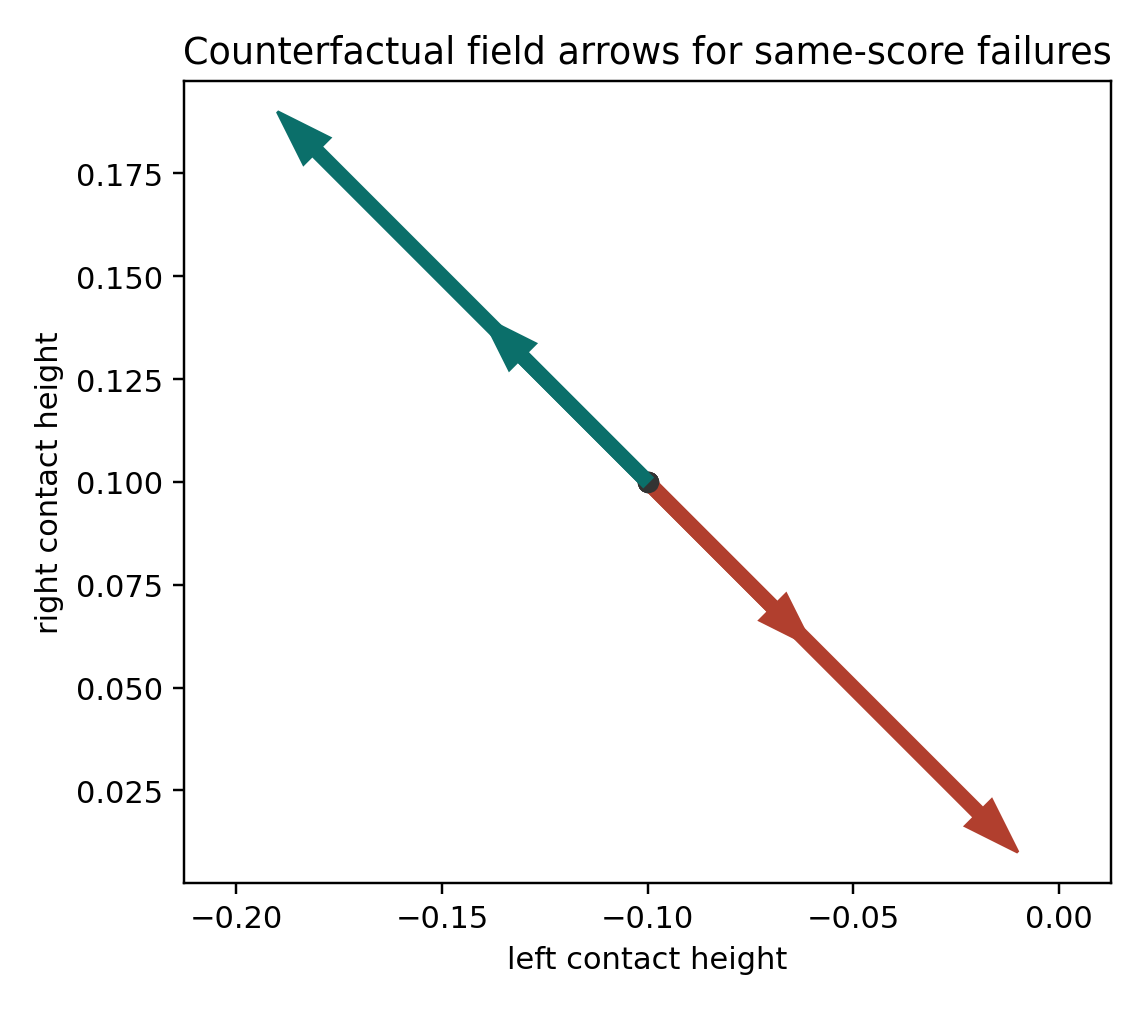
\includegraphics[width=0.68\linewidth]{figures/pair_failure_fields.png}
    \caption{Original same-score pair field arrows. Points with equal scalar failure scores can require opposite signed edits in contact space. The figure is retained because it makes the proposition visually auditable.}
    \label{fig:pair-fields}
\end{figure}

The original same-score pairs are intentionally small. For two selected absolute errors, the script creates one state with positive wrench-balance error and one state with negative error. The scalar score is a function of $|e|$, so the paired states are indistinguishable to a scalar magnitude representation. The field arrows in Figure~\ref{fig:pair-fields} point in opposite directions. This is the whole scalar-insufficiency argument in one picture.

The full-scale linear family adds a second kind of case study. In multi-contact states, two failures can have the same signed error but different leverage and cost structure. A signed scalar tells the controller which side of the interval to move toward, but it does not tell the controller which contact should move. If contact 1 has high leverage but high cost, contact 2 has lower leverage but low cost, and contact 3 is near its limit, the minimum field can be a distributed edit. Uniform signed repair ignores that structure. Nearest-contact repair captures only one part of it.

The mask/limit suite adds a third case. Some failed states have a mathematically clear desired balance change but no feasible active-contact edit. In those cases, the right field output is not a vector pretending to solve the problem. It is an infeasibility certificate. A robot can use that certificate to open the gripper, change contact set, or switch to a different repair mode.

These case types are why the paper uses the word ``field'' rather than ``signed error.'' The signed error is enough in the simplest unconstrained linear projection. The field is the contact-indexed object that remains meaningful when contact weights, costs, masks, limits, and feasibility matter.

\clearpage
\section{Appendix I: Baseline Failure Ledger}

This appendix records what each baseline teaches. It is included to prevent the results from collapsing into a single leaderboard.

\paragraph{No repair.}
No repair succeeds in 0.0\% of the sampled failed states. This confirms that the generators are not accidentally mixing in already stable grasps. It also sets the semantic baseline: every success reported by a repair method comes from moving contact variables, not from a loose success predicate.

\paragraph{Scalar random sign.}
Scalar random sign is the cleanest test of missing direction. In the original 20,000-case experiment it succeeds in 50.59\%. In the linear contact grid it succeeds in 48.9\%, and in the large stress suite it succeeds in 46.9\%. The small deviations from 50\% come from clipping, masks, and finite sampling. The baseline is intentionally generous because it knows the repair magnitude and uses a contact-allocation routine after guessing sign.

\paragraph{Scalar global sign.}
Scalar global sign shows the danger of biased data. In the balanced linear grid it is near chance. In the biased grid it can reach high average success by always choosing the majority direction. At a 0.95 positive prior it reaches 95.1\% average success and 0.0\% worst-group success. This is the most review-relevant scalar failure because it resembles an empirical classifier that learns the dataset prior rather than the realized contact repair.

\paragraph{Scalar prior sample.}
Scalar prior sampling is less degenerate than global sign because it sometimes chooses the minority direction. But it still does not condition on the state. At the 0.95 prior, its worst-group success is 7.9\%. The result says that matching the marginal action distribution is not enough for contact repair.

\paragraph{Uniform signed repair.}
Uniform signed repair receives the correct sign, so it is not a scalar magnitude-only baseline. Its failures show that sign is not allocation. It spends more effort than the field in the stress suite and succeeds less often. The baseline is useful because it isolates the step from ``which way'' to ``which contacts and how much.''

\paragraph{Nearest-contact repair.}
Nearest-contact repair is a strong heuristic. It reaches 91.6\% success in the feasible linear grid and 79.4\% in the large stress suite. Its failures are not random. They occur when the best single contact clips, when several contacts must share the edit, or when the highest leverage contact is not the lowest cost contact. It is a serious baseline because many real controllers prefer sparse corrective moves.

\paragraph{Noisy signed margin.}
Noisy signed margin tests the gap between analytic mechanics and estimated mechanics. The exact signed margin is sufficient in the linear model, but noisy estimates are not. The current one-step metric is harsh because the projection targets the boundary. This baseline therefore motivates uncertainty-aware fields rather than weakening the field claim.

\paragraph{Signed-margin projection.}
Signed-margin projection is the upper bound. It matches the field whenever the field is feasible because both solve the same constrained projection. Reporting this result is essential: the paper is not claiming that a new representation beats calibrated mechanics. It claims that calibrated mechanics should be represented as an executable field, not reduced to a scalar label.

\paragraph{Counterfactual field.}
The field succeeds exactly when the constrained projection is feasible and the model is exact. In the large stress suite it succeeds in 96.0\%, with the remaining cases explained by field infeasibility. The key advantage is not numerical dominance over signed margin. It is auditability: direction, allocation, effort, and infeasibility are explicit.

\clearpage
\section{Appendix J: Metric Rationale}

\paragraph{Why not only average success?}
Average success can be gamed by repair-sign bias. The scalar global-sign baseline is the canonical example: it reaches high average success as one repair direction dominates, while worst-group success remains 0.0\%. For grasp repair, the rare direction may correspond to a rare object pose, a rare slip mode, or a less common contact arrangement. Those failures are operationally important.

\paragraph{Why balanced success?}
Balanced success averages success on positive and negative repair directions. It asks whether the method repairs both sides of the failure boundary. In a balanced dataset, average and balanced success are similar. In a biased dataset, the gap reveals whether the method learned a state-conditioned repair or only a population prior.

\paragraph{Why worst-group success?}
Worst-group success is the stricter version of balanced success. It captures the failure mode that matters for deployment: one repair direction may be systematically broken even when the average looks high. In this paper, worst-group success exposes the scalar global-sign baseline immediately.

\paragraph{Why effort?}
A method can succeed by issuing large contact edits. The field minimizes a weighted repair norm, so effort is part of the object. Uniform signed repair often spends more effort than the field because it ignores leverage and cost. A real robot would also care about object disturbance, contact risk, and gripper motion; effort is the simplified proxy used here.

\paragraph{Why infeasibility?}
Infeasibility is not the same as repair failure. If no active-contact edit can cross the success boundary within limits, a one-step field should report that fact. A scalar failure label cannot distinguish ``the repair direction is unknown'' from ``the required repair cannot be executed.'' This distinction is important for deciding whether to continue tactile servoing or regrasp.

\paragraph{Why post-repair margin?}
The one-step field targets the boundary in the exact model. This makes post-repair margin near zero for oracle field methods and reveals sensitivity to noise. A robust hardware method should add slack; the current metric intentionally exposes the boundary-targeted nature of the analytic projection.

\clearpage
\section{Appendix K: Stress Suite Reading Guide}

The large stress suite combines multiple axes of variation. It should not be read as a claim that the linear model is realistic. It should be read as a compact adversarial audit of the representation.

\paragraph{Contact count.}
The suite uses two to six contact coordinates. Two contacts preserve the spirit of the original pinch. More contacts test whether the repair object carries allocation information. Scalar sign baselines do not know allocation; uniform and nearest-contact baselines use simple allocation heuristics; the field computes the weighted constrained allocation.

\paragraph{Repair-sign prior.}
The stress suite mixes sign priors. This prevents the headline from depending only on balanced data. The global scalar baseline benefits from biased priors in average success, but its worst-group success remains poor.

\paragraph{Active-contact masks.}
Masks represent contacts that cannot be moved or trusted for a repair step. In hardware, this could be a finger at a kinematic limit, a tactile patch without controllable shear, or a contact that would collide if moved. Masks turn some otherwise valid fields into infeasible repairs.

\paragraph{Travel limits.}
Travel limits represent local action bounds. Even if a contact has the right leverage, it may not be able to move far enough. The active-set projection clips contacts that hit their bounds and continues with the remaining contacts. If the required balance change remains unreachable, the field is infeasible.

\paragraph{Near-limit states.}
Some stress cases deliberately sample contacts near their limits. This increases infeasibility and makes greedy nearest-contact repair less reliable. It is a synthetic proxy for already-loaded grasps where the controller has little remaining contact motion.

\paragraph{Noise.}
The stress suite includes noise settings, but the exact signed-margin and field baselines remain oracle references. The separate noise grid is the better place to read estimation brittleness. The stress suite's role is to show how the representation behaves when several non-idealities are mixed.

\paragraph{Main reading.}
The stress result should be summarized as follows: scalar magnitude methods lose direction; majority scalar methods can hide minority failure; sign-only methods lose allocation; greedy allocation is strong but incomplete; exact signed mechanics and the field match when feasible; field infeasibility is the boundary that should trigger a different behavior.

\clearpage
\section{Appendix L: From Analytic Fields To Learned Repair Targets}

The full-scale experiments are analytic, but the representation is intended to be useful for learned tactile repair. This appendix spells out what would change if the field were used as a supervision target.

\paragraph{Labeling target.}
A scalar dataset records something like $(o,a,y)$, where $o$ is an observation, $a$ is a grasp action, and $y\in\{0,1\}$ or $y\in[0,1]$ is the outcome. A field dataset would instead record $(o,a,\Delta^\star,\eta)$, where $\Delta^\star$ is a contact edit or repair set and $\eta$ records feasibility or confidence. The field can be produced by analytic mechanics, an offline optimizer, human demonstration, repeated probing, or a local tactile servoing routine. The important point is that the label is an action object, not only an outcome.

\paragraph{Loss functions.}
A learned field predictor should not be evaluated only by mean squared vector error. It should also be evaluated by repaired-state success, effort, constraint violation, and worst-group success over repair directions. If several repairs are equivalent, a single vector loss can penalize a valid alternative. In that case the target should be a set, distribution, or energy over executable repairs.

\paragraph{Ambiguity.}
The analytic linear model uses weighted Euclidean cost, which makes the field unique. Real grasps often admit multiple repairs: move the left finger, move the right finger, increase normal force, roll the object slightly, or regrasp. A learned system should expose this ambiguity. Collapsing all alternatives into one average vector can produce a repair that is physically meaningless.

\paragraph{Confidence and infeasibility.}
The field target should include whether a repair is feasible under the current contacts. If the offline optimizer cannot find a one-step repair, that is still a useful label. It tells the policy to change contact set or retreat. This is why the mask/limit suite reports field infeasibility instead of counting every infeasible case as an ordinary failed repair.

\paragraph{Policy integration.}
A field predictor can be used as a one-step command, as a proposal for a model predictive controller, or as a target for a tactile servoing loop. The paper does not choose among these. The representational claim is upstream: regardless of controller, the repair target should preserve contact direction, allocation, effort, and feasibility.

\paragraph{Why scalar pretraining is not enough.}
A scalar success model can still be useful as a filter or uncertainty signal. It can say that a grasp is bad. But unless it is paired with signed contact information and an action model, it does not say how to repair the grasp. The biased scalar experiment shows how a scalar model can look good by learning the common repair direction while failing rare directions.

\paragraph{Minimum dataset report.}
A future learned-field paper should report at least: distribution of repair signs, distribution of repair efforts, fraction of non-unique or infeasible repairs, success after executing predicted repairs, balanced success over repair directions, and performance on rare contact modes. Without those reports, a scalar or vector policy can hide the same ambiguity this paper exposes.

\clearpage
\section{Appendix M: Non-Unique Fields, Costs, And Repair Sets}

The paper uses a weighted Euclidean cost because it gives a clean projection. That choice is not universal. A real robot may care about maximum finger motion, object disturbance, normal-force increase, tactile shear, collision risk, or energy. Different costs produce different counterfactual fields.

\paragraph{Cost dependence.}
If the cost is
\begin{equation}
    \cost_2(\delta)=\sum_i c_i\delta_i^2,
\end{equation}
the linear projection distributes motion according to $w_i/c_i$. If the cost is
\begin{equation}
    \cost_1(\delta)=\sum_i c_i|\delta_i|,
\end{equation}
the minimum often concentrates on one or a few contacts. If the cost is maximum motion,
\begin{equation}
    \cost_\infty(\delta)=\max_i |\delta_i|,
\end{equation}
the minimum can spread motion to equalize the largest displacement. These are different repair objects, even for the same failed state.

\paragraph{Repair sets.}
When multiple repairs have the same cost, the right object is a set:
\begin{equation}
    \field(\state)=
    \{\delta\in\actions(\state): \state+\delta\in\success,\ \cost(\delta)=\cost^\star\}.
\end{equation}
Reporting only one arbitrary member of the set can hide useful alternatives. For example, if two contacts have identical leverage and cost, either contact can supply the same balance change. A controller with local tactile uncertainty may prefer the contact with higher confidence, even if both are mechanically equivalent.

\paragraph{Why this matters for learning.}
If a dataset chooses one repair from a non-unique set and trains a regressor with squared error, the learned model may average incompatible alternatives. A repair-set target or conditional generative model is better aligned with the physics. The field representation naturally accommodates this by treating the counterfactual as an action object rather than a scalar outcome.

\paragraph{Why the present paper keeps a unique cost.}
The goal here is to isolate scalar insufficiency, not to solve general contact optimization. A unique weighted projection removes one source of ambiguity so that direction, allocation, and feasibility can be studied cleanly. The appendices make clear that richer costs are a future expansion, not something hidden by the current experiments.

\paragraph{Evaluation implication.}
For non-unique fields, exact vector match is the wrong metric. A predicted repair should be judged by whether it belongs to the feasible repair set, how much cost gap it has relative to the minimum, and whether it succeeds when executed. This is another reason the full-scale tables emphasize repaired-state success, effort, and infeasibility instead of only vector error.

\clearpage
\section{Appendix N: Artifact Map}

\begin{center}
\scriptsize
\resizebox{\linewidth}{!}{%
\begin{tabular}{@{}lp{0.70\linewidth}@{}}
\toprule
Artifact & Purpose \\
\midrule
\texttt{src/cgff\_mechanics.py} & Original symmetric pinch mechanics. \\
\texttt{experiments/run\_counterfactual\_fields.py} & Original 20,000-case and 30-seed stress experiment. \\
\texttt{experiments/run\_full\_scale\_fields.py} & Full-scale streamed linear contact-balance suites and summarize-only path. \\
\texttt{results/counterfactual\_field\_summary.json} & Original main summary. \\
\texttt{results/stress\_summary.json} & Original 30-seed stress summary. \\
\texttt{results/full\_scale/full\_scale\_summary.json} & Full-scale suite sizes and streaming metadata. \\
\texttt{results/full\_scale/leaderboard.csv} & Full-scale aggregate metrics by suite and baseline. \\
\texttt{paper/figures/} & Paper-ready generated figures. \\
\texttt{paper/tables/} & Generated LaTeX table fragments. \\
\texttt{docs/full\_scale\_execution\_plan.md} & Per-paper execution plan written before full-scale edits. \\
\bottomrule
\end{tabular}
}
\end{center}

\section{Appendix O: What A Hardware Version Would Need}

A hardware version would need at least five additions.

\paragraph{Tactile contact-state estimation.}
The robot would need estimates of contact locations, normals, local slip, and force/traction distributions with uncertainty. The present paper assumes the contact state is available.

\paragraph{Friction-cone and wrench constraints.}
The linear balance interval should be replaced with friction-cone, wrench-space, and object-pose constraints. The field would become a constrained optimization over contact patches and forces.

\paragraph{Action feasibility.}
The action set should include gripper kinematics, tactile patch motion limits, collision constraints, and object motion induced by the repair.

\paragraph{Robustness.}
The noisy-margin result shows that boundary-targeted one-step repair is brittle. Hardware fields should include slack, uncertainty, and feedback after partial edits.

\paragraph{Evaluation.}
The main metric should not only be grasp success after repair. It should include field feasibility, repair effort, minority-direction success, object disturbance, and whether the predicted field matches an independently solved or demonstrated repair.

\clearpage
\section{Appendix P: Design Requirements From The Negative Results}

The negative results in this paper are not side notes. They are design requirements for any system that tries to use failure fields in a robot.

\paragraph{Report direction-conditioned performance.}
The biased scalar grid shows that average success can be misleading. Any learned repair system should report performance separately by repair direction or by mechanically meaningful contact mode. If the minority direction is rare, the evaluation set should rebalance it or report worst-group success.

\paragraph{Separate sign, allocation, and feasibility.}
The baseline ladder shows three different information losses. Scalar magnitude loses sign. Uniform signed repair has sign but loses allocation. Greedy nearest-contact repair has a simple allocation but not the constrained minimum. Field infeasibility is a fourth category. A useful benchmark should report which of these failures occurred.

\paragraph{Expose contact masks.}
Real contact sets change. A tactile patch may lose contact, a finger may be at a limit, or a collision constraint may remove an action. The mask/limit suite shows that a field is only meaningful relative to the currently executable action set. A system that predicts a repair vector without an action mask can propose impossible repairs.

\paragraph{Use slack under uncertainty.}
The noisy signed-margin result is a warning about boundary-targeted one-step repair. If estimates are noisy, reaching the exact boundary is not robust. A practical controller should target a positive margin, re-estimate after partial motion, or represent uncertainty in the field.

\paragraph{Keep the field auditable.}
The field should be stored with its cost, feasibility status, post-repair margin, and active constraints. Without this audit trail, a field predictor becomes another black-box action policy and loses the main advantage of the representation.

\bibliographystyle{iclr2026_conference}
\bibliography{references}

\end{document}
